\documentclass[18pt, twoside]{article}
\usepackage[utf8]{inputenc}
\usepackage{polski}
\usepackage{graphicx}
\graphicspath{ {./images/} }
\usepackage[margin=0.5in]{geometry}


\begin{document}
\begin{figure}[tp!]
\center{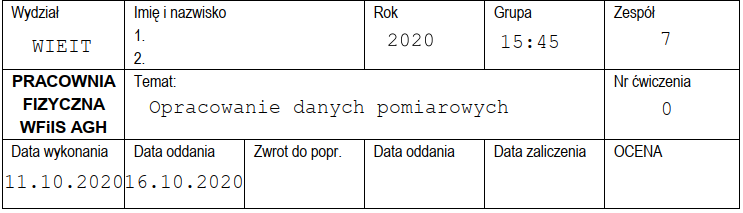
\includegraphics{F}}
\end{figure}

\begin{center}
    \section*{Opracowanie Danych Pomiarowych}
    \emph{Dzmitry Mikialevich}
\end{center}
\begin{center}
    \emph{Wojciech Sikora}
\end{center}
\tableofcontents
\newpage

\section{Wstęp}
\subsection{Cel ćwiczenia}
 % Tu TEKST
\subsection{Opis ćwiczenia}
 % Tu TEKST
\section{Układ Pomiarowy}
 % Tu TEKST
\section{Przebiegi doświadczenia}
 % Tu TEKST
\section{Wyniki Pomiarów}

{
     \begin{table}[h]
     \centering
    \begin{tabular}{|l|l|l|l|}
    \hline

    Lp.& Liczba okresów k & Czas t dla k okresów \([s]\)  & okres \(T_i = t/k \)  \([s]\)   \\ \hline
    1 & 10  & 11.72  & 1.172 \\ \hline
    2 & 10  &  12.12 & 1.212 \\ \hline
    3 & 10  &  12.42 &  1.242 \\ \hline
    4 & 10  &  11.87 &  1.187 \\ \hline
    5 & 10  &  11.88 &  1.188 \\ \hline
    6 & 10  &  11.78 &  1.178 \\ \hline
    7 & 10  &  11.84 &  1.184 \\ \hline
    8 & 10  &  11.85 &  1.185 \\ \hline
    9 & 10  &  11.87 &  1.187 \\ \hline
    10 & 10  &  11.95 &  1.195 \\ \hline
    \end{tabular}
    \textbf{\caption{Pomiar okresu drgań przy ustalonej długości wahadła  }
}
\end{table}}


{
     \begin{table}[h]
     \centering
    \begin{tabular}{|l|l|l|l|l|l|}
    \hline
    Lp. & l \([mm]\) & \(k\) & \(t[s]\) & \(T_i[s]\) &  \(T_i^2[s^2]\) \\ \hline
    1 &  &  &  &  &\\ \hline
    2 &  &  &  &  &\\ \hline
    3 &  &  &  &  &\\ \hline
    4 &  &  &  &  &\\ \hline
    5 &  &  &  &  &\\ \hline
    6 &  &  &  &  &\\ \hline
    7 &  &  &  &  &\\ \hline
    8 &  &  &  &  &\\ \hline
    9 &  &  &  &  &\\ \hline
    10 &  &  &  &  &\\ \hline
    11 &  &  &  &  &\\ \hline
    12 &  &  &  &  &\\ \hline
    13 &  &  &  &  &\\ \hline
    14 &  &  &  &  &\\ \hline
    15 &  &  &  &  &\\ \hline
    \end{tabular}
    \textbf{\caption{Pomiar zależności okresu drgań od długości wahadła }
}
\end{table}}
 

 
 
 
\section{Opracowanie wyników Pomiarów}
\subsection{Błędy grube}
 % Tu TEKST
\subsection{Niepewność pomiaru okresu (typu A)}
 % Tu TEKST
 \subsection{Niepewność pomiaru długości wahadła (typu B)}
 % Tu TEKST
 \subsection{Przyspieszenie ziemskie  na podstawie uzyskanych wartości \(l\) i \(T\)}
 % Tu TEKST
 \subsection{Niepewność złożoną \(u_c(g)\) przy pomocy prawa przenoszenia niepewności}
 % Tu TEKST
 \subsection{Niepewność rozszerzoną \(U(g)\)) przy pomocy prawa przenoszenia niepewności}
 % Tu TEKST
 \subsection{Porównanie uzyskanej wartości przyspieszenia ziemskiego z wartością tabelaryczną}
 % Tu TEKST
 \subsection{wykres zależności okresu od długości wahadła \(T(l)\)}
 % Tu TEKST
 \subsection{Wykres zlinearyzowany \(T^2\) w funkcji l}
 % Tu TEKST
 \subsection{Dopasowanie prostej typu \(y = ax\)}
 % Tu TEKST
 \subsection{Wartość przyspieszenia 
ziemskiego z otrzymanej wartości współczynnika nachylenia}
 % Tu TEKST
 \subsection{Obliczanie niepewności u(g) z niepewności u(a) }
 % Tu TEKST
\section{Wnioski}
\subsection{elo}
 % Tu TEKST
Lorem ipsum dolor sit amet, consectetuer adipiscing elit.  
Etiam lobortis facilisissem.  Nullam nec mi et neque pharetra 
sollicitudin.  Praesent imperdiet mi necante...


\end{document}